\section{System Design and Demo Walkthrough}
\label{sec:system}

\begin{figure*}[t]
\centering
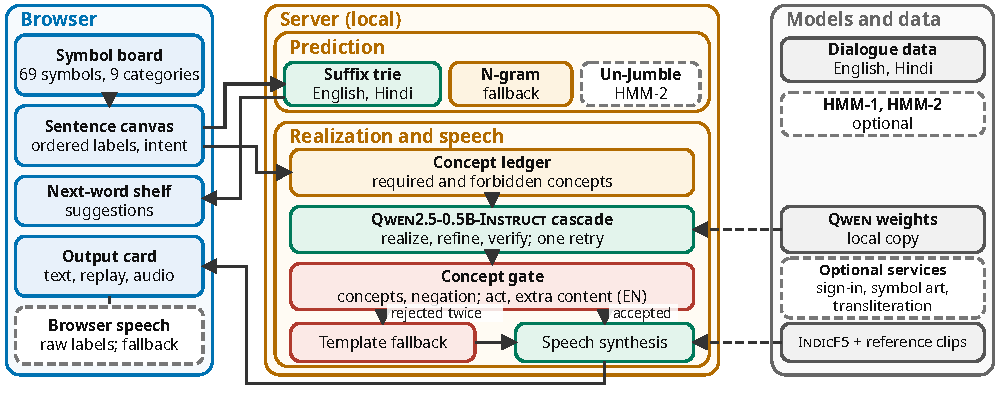
\includegraphics[width=0.92\textwidth]{figures/architecture.pdf}
\caption{Architecture of \sys{}; dashed boxes are optional. The cascade output is spoken only if the gate accepts it, and a template fallback is spoken after two rejections.}
\label{fig:arch}
\end{figure*}

\paragraph{Walkthrough.}
Figure~\ref{fig:arch} shows the decision path from a selection to the spoken sentence.
The user picks a language and taps symbols from a board of \NSymbols{} symbols in \NCategories{} categories, labeled in English, Hindi, Gujarati, and Marathi (Figure~\ref{fig:ui}, \cn{1}).
Selections accumulate on a sentence canvas (\cn{2}), and a shelf proposes next words with their probabilities (\cn{3}).
\emph{Speak} voices the literal labels with the browser's speech synthesis; \emph{AI Polish \& Speak} (\cn{4}) sends the selection to the server, which returns a sentence that the output card shows while it is spoken (\cn{5}).
\emph{Quick Express} speaks emergency phrases in one tap, and \emph{Un-Jumble} reorders canvas words with a second hidden Markov model (HMM).

\begin{figure}[t]
\centering
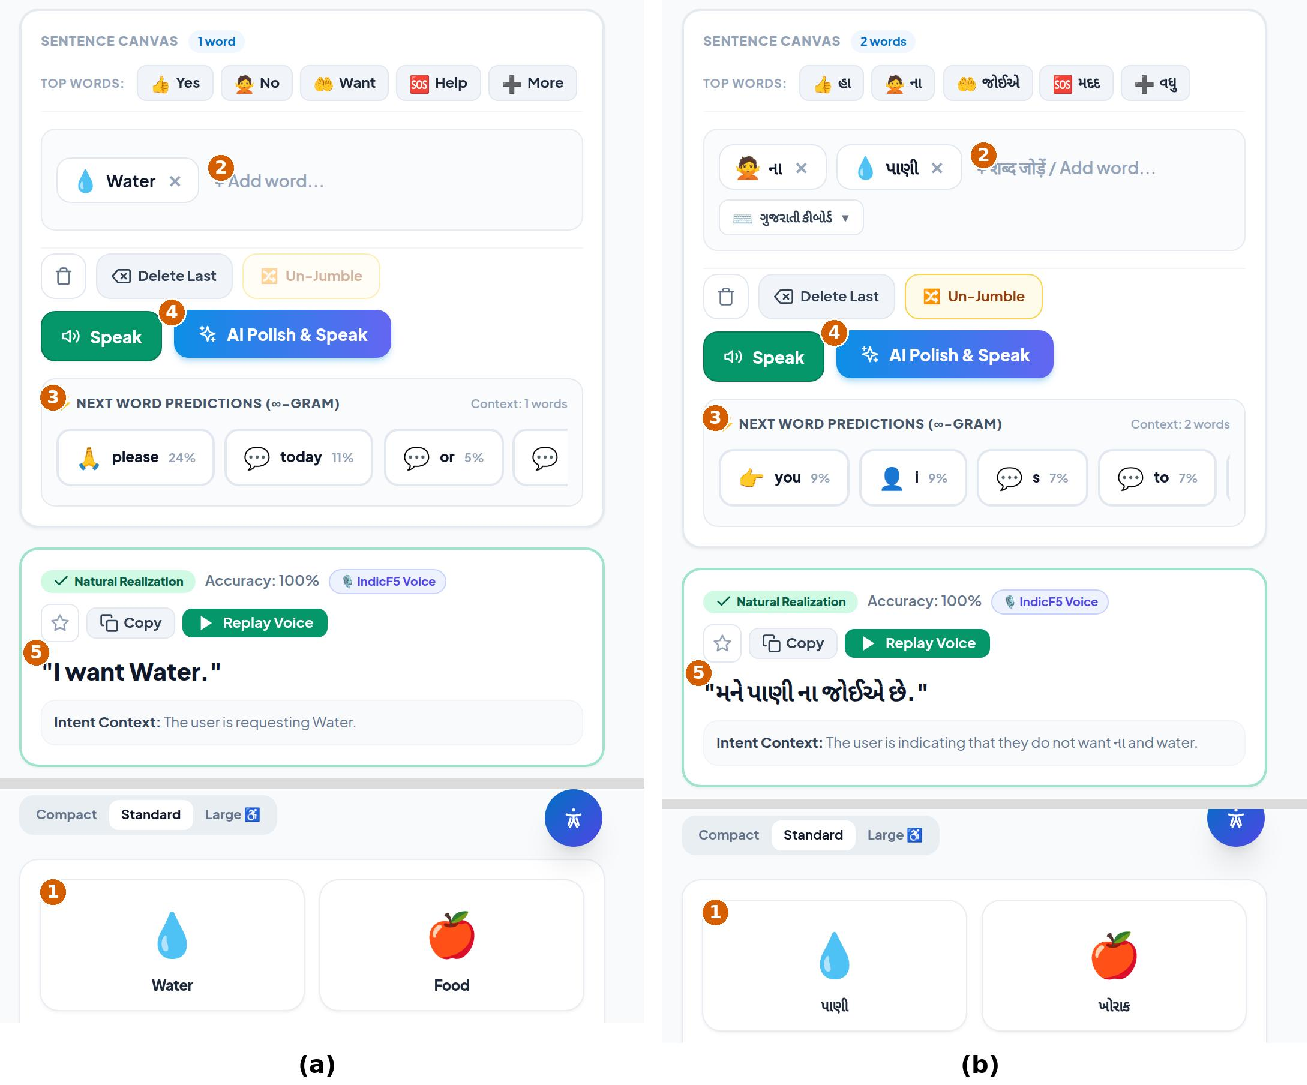
\includegraphics[width=0.9\columnwidth]{figures/ui_panel.pdf}
\caption{The evaluated build (the repaired build adds route chips, a message-type control, and a clarification card; Section~\ref{sec:repair}). (a)~English \emph{Water}: cascade output rejected, template fallback spoken. (b)~Gujarati \gu{ના}\,+\,\gu{પાણી}: cascade output accepted. The voice chip reads ``IndicF5 Voice'' although the server returned a placeholder tone; the \emph{Accuracy} badge is not used by the gate.}
\label{fig:ui}
\end{figure}

\paragraph{Input and concept ledger.}
The browser sends the ordered labels with the communicative intent (request, statement, question, or negation), a negation indicator, the language, and an optional code-mixing indicator.
The evaluated client infers intent and negation from label substrings (a negator in a label means negation, question words a question, a few feeling labels a statement, anything else a request); any other client can supply both fields explicitly, the explicit condition of Section~\ref{sec:eval}.
The server builds the ledger: a required set (intent, speaker, each selected concept, negation) and a forbidden set of 21 default words for unrequested times, meals, and venues, minus any word the user selected.

\paragraph{Realization and gate.}
Three prompted stages share one frozen \qwen{}.
The realizer writes a sentence from a few-shot prompt for Hindi, Gujarati, and Marathi (12, 9, and 9 examples; greedy decoding) and from a ledger prompt for English and code-mixed output (temperature 0.1).
The refiner removes unsupported content and is skipped for Indic-script candidates; the verifier returns a verdict, which is unused, and a minimal rewrite, which changed English candidates but no Indic one.
The gate decides by Equation~\eqref{eq:gate}, with $\nu$ the negation indicator, $E$ the selected concepts, $F$ the forbidden set, and $y$ the candidate:
\begin{equation}
\begin{split}
\mathrm{acc}(y)={}&[\mathrm{neg}(y)=\nu]\wedge\mathrm{match}(E,y)\wedge\mathrm{act}(y)\\
&\wedge\neg\mathrm{forbid}(y)\wedge\neg\mathrm{time}(y).
\end{split}
\label{eq:gate}
\end{equation}
Here \emph{neg} tests lists of English, Hindi, Gujarati, and Marathi negators; \emph{match} requires every selected concept to appear ; \emph{act} rejects ``I want'' for a feeling and requires a question cue for a question; \emph{forbid} matches a word of $F$; and \emph{time} flags time words when none was selected.
The act cues and the word lists are English only, so for Hindi, Gujarati, and Marathi the gate tests concept presence and negation.
A rejection triggers one more cascade run, and after two rejections a language-specific template fallback built from the selected labels (e.g., ``I want Water.'') is returned; English retries resample, whereas greedy Indic retries repeat the first output.

\paragraph{Prediction, speech, and training.}
Next-word suggestions come from an unbounded-order suffix trie in the spirit of infini-gram \citep{liu2024infinigram}, built at start-up from the English and Hindi AAC dialogues (\IGSent{} sentences, maximum depth \IGDepth{}).
Marathi reuses the Hindi trie and Gujarati has no predictor; two HMMs trained on streamed text (HMM-1 for next words, HMM-2 for Un-Jumble) are optional and were absent from the evaluated build.
The returned sentence is synthesized by \indicf{} \citep{ai4bharat2025indicf5}, a flow-matching model of the F5-TTS family \citep{chen2025f5tts}, with a 24\,kHz \vocos{} vocoder \citep{siuzdak2023vocos}, conditioned zero-shot on a reference clip and its transcript; the default clip is a Punjabi recording sent for every language, and an English narrator clip can be selected.
The model card lists Hindi, Gujarati, and Marathi but not English, so English speech is unverified.
Browser speech voices the literal labels and replaces server audio only when none is returned (Appendix~\ref{app:coverage}).
In the evaluated build no route produced speech: the gated weights were absent, so the server returned a placeholder tone that the client played, and headless Chrome exposed no voices.
We train the suffix trie, four HMMs, and an English \flant{} refiner (Appendix Table~\ref{tab:models}).
